\documentclass[12pt,a4paper]{article}
\usepackage{amsmath}
\usepackage{mathtext}
\usepackage{icomma}
\usepackage{amsfonts}
\usepackage{amssymb}
\usepackage[utf8]{inputenc}
\usepackage[T1,T2A]{fontenc}
\usepackage[english, russian]{babel}
\usepackage{graphicx}
\usepackage[left=2cm,right=2cm,top=2cm,bottom=2cm]{geometry}
\usepackage{calc}
\usepackage{wrapfig}
\usepackage{setspace}
\usepackage{indentfirst}
\usepackage{subfigure}
\usepackage[table,xcdraw]{xcolor}
\usepackage{float}

\title{
Отчет о выполнении лабораторной работы 3.2.1 \\
Сдвиг фаз в цепи переменного тока.}

\author{Фитэль Алёна, Попеску Полина\\ группа Б06-103}

\begin{document}

\maketitle

\subparagraph*{Аннотация.} В работе исследована зависимость сдвига фаз между током и напряжением от сопротивления в $RC -$ и в $RL - $ цепи;
определена добротность колебательного контура путем снятия зависимости сдвига фаз от частоты вблизи резонанса; 
оценен диапазон работы фазовращателя.

\subsection*{Теоретическое введение}

Удобным, хотя и не очень точным прибором для измерения фазовых соотношений служит электронный осциллограф. 
Пусть нужно измерить сдвиг фаз между двумя напряжениями $U_1$ и $U_2$. 
Подадим эти напряжения на горизонтальную и вертикальную развёртки осциллографа. 
Смещение луча по горизонтали и вертикали определяется выражениями $$x = x_0 \cos \Omega t,\quad y = y_0 \cos (\Omega t + \alpha),$$ где $\alpha$ — сдвиг фаз между напряжениями $U_1$ и $U_2$, а $x_0$ и $y_0$ — амплитуды напряжений, умноженные на коэффициенты усиления соответствующих каналов осциллографа. 
Исключив время, после несложных преобразований найдём:
\begin{equation*}
    \left( {x \over x_0}\right)^2 + \left( {y \over y_0}\right)^2 + {2xy \over x_0y_0} \cos \alpha = \sin^2 \alpha.
\end{equation*}
\hfill
\begin{wrapfigure}{l}{0.4\linewidth}
    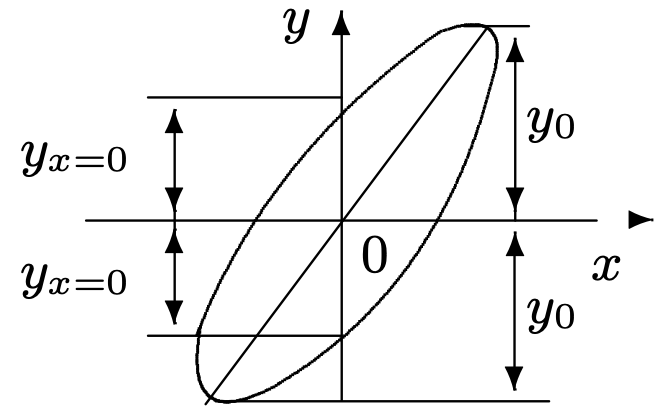
\includegraphics[width=\linewidth]{ellipse.png}
    \caption{Эллипс на экране осциллографа}
\end{wrapfigure}

Полученное выражение определяет эллипс, описываемый электронным лучом на экране осциллографа (рис. 1). 
Ориентация эллипса зависит как от искомого угла $\alpha$, так и от усиления каналов осциллографа. 
Для расчёта сдвига фаз можно измерить отрезки $2y_{x=0}$ и $2y_0$ (или $2x_{y=0}$ и $2x_0$, на рисунке не указанные) и, подставляя эти значения в уравнение эллипса, найти $$\alpha = \pm \arcsin \left({y_{x=0} \over y_0}\right).$$

Для правильного измерения отрезка $2y_{x=0}$ важно, чтобы центр эллипса лежал на оси y.

\newpage

\begin{wrapfigure}{l}{0.3\linewidth}
    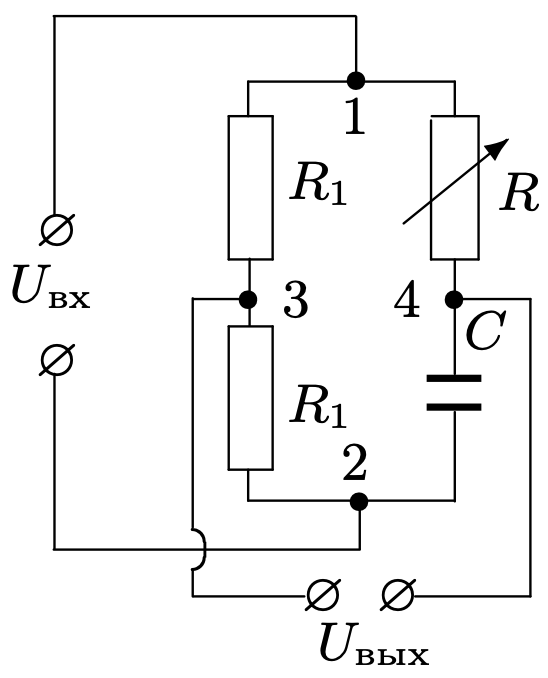
\includegraphics[width=0.8\linewidth]{phase.png}
    \caption{Принципиальная схема фазовращателя}
\end{wrapfigure}
Другой способ измерения сдвига фаз изложен в описании экспериментальной установки.

На практике часто используются устройства, позволяющие в широких пределах изменять фазу напряжения ($0 < \psi < \pi$). 
Такие устройства называются фазовращателями. 
Схема простого фазовращателя приведена на рис. 2. 
Она включает в себя два одинаковых резистора $R_1$, ёмкость $C$ и переменное сопротивление $R$.

Используя метод комплексных амплитуд, найдём зависимость сдвига фаз между входным напряжением  \\ $U_{вх} = U_0 \cos \Omega t$ и выходным $U_{вых}$ от соотношения между импедансами сопротивления $R$ и ёмкости $C$. 
Для этого выразим выходное напряжение $U_{вых}$ через $U_вх$, параметры контура и частоту внешнего источника $\Omega:\ U_{34} = f(U_{12},\ R,\ C,\ \Omega)$.

Обозначим комплексную амплитуду входного напряжения через $\widehat{U}_0$. 
Тогда напряжение между точками 1 и 3 в силу равенства сопротивлений $R_1$ $$\widehat{U}_{13} = {\widehat{U}_0 \over 2}.$$
Если фазу напряжения $\widehat{U}_{вх}$ положить равной нулю, то $\widehat{U}_0$ будет действительной величиной: $\widehat{U}_0 = U_0$. Приняв напряжение в точке 1 равным нулю, получим амплитуду напряжения в точке 3: $$\widehat{U}_{03} = {U_0 \over 2}.$$
Расчитаем $\widehat{U}_{04}$ -- амплитуду напряжения в точке 4. 
Импеданс $Z$ последовательно соединённых сопротивления $R$ и ёмкости $C$ равен $$Z = R - {i \over \Omega C}.$$
Для комплексной амплитуды тока $$\widehat{I}_0 = {U_0 \over Z} = {U_0 \over R - i/\Omega C},$$ 
а для комплексной амплитуды напряжения в точке 4 -- $$\widehat{U}_{04} = \widehat{I}_{0}R = U_0 {R \over R - i/\Omega C}.$$
Выходное напряжение $$\widehat{U}_{вых} = \widehat{U}_{04} - \widehat{U}_{03} = \widehat{U}_{04} - U_0/2 = {U_0 \over 2} { R + i/\Omega C \over R - i/\Omega C}.$$

В числитель и знаменатель последнего выражения входят комплексно-сопряжённые выличины, модули которых одинаковы, поэтому величина выходного напряжения не меняется при изменении $R$.
Модуль $U_{вых}$ всегда равен $U_0 / 2$ -- половине $U_{вх}$.
Сдвиг фаз между входным и выходным напряжениями равен $2\arctan(1/\Omega RC)$ и меняется от $\pi$ (при $R \longrightarrow 0$) до $0$ (при $R \longrightarrow \infty$).

\newpage
\subsection*{Экспериментальная установка}

Схема для исследования сдвига фаз между током и напряжением в цепи переменного тока представлена на рис. 3.
Эталонная катушка $L$, магазин емкостей C и магазин сопротивлений $R$ соединены последовательно и через дополнительное сопротивление $r$ подключены к источнику синусоидального напряжения — звуковому генератору.

\begin{figure}[h]
    \centering
    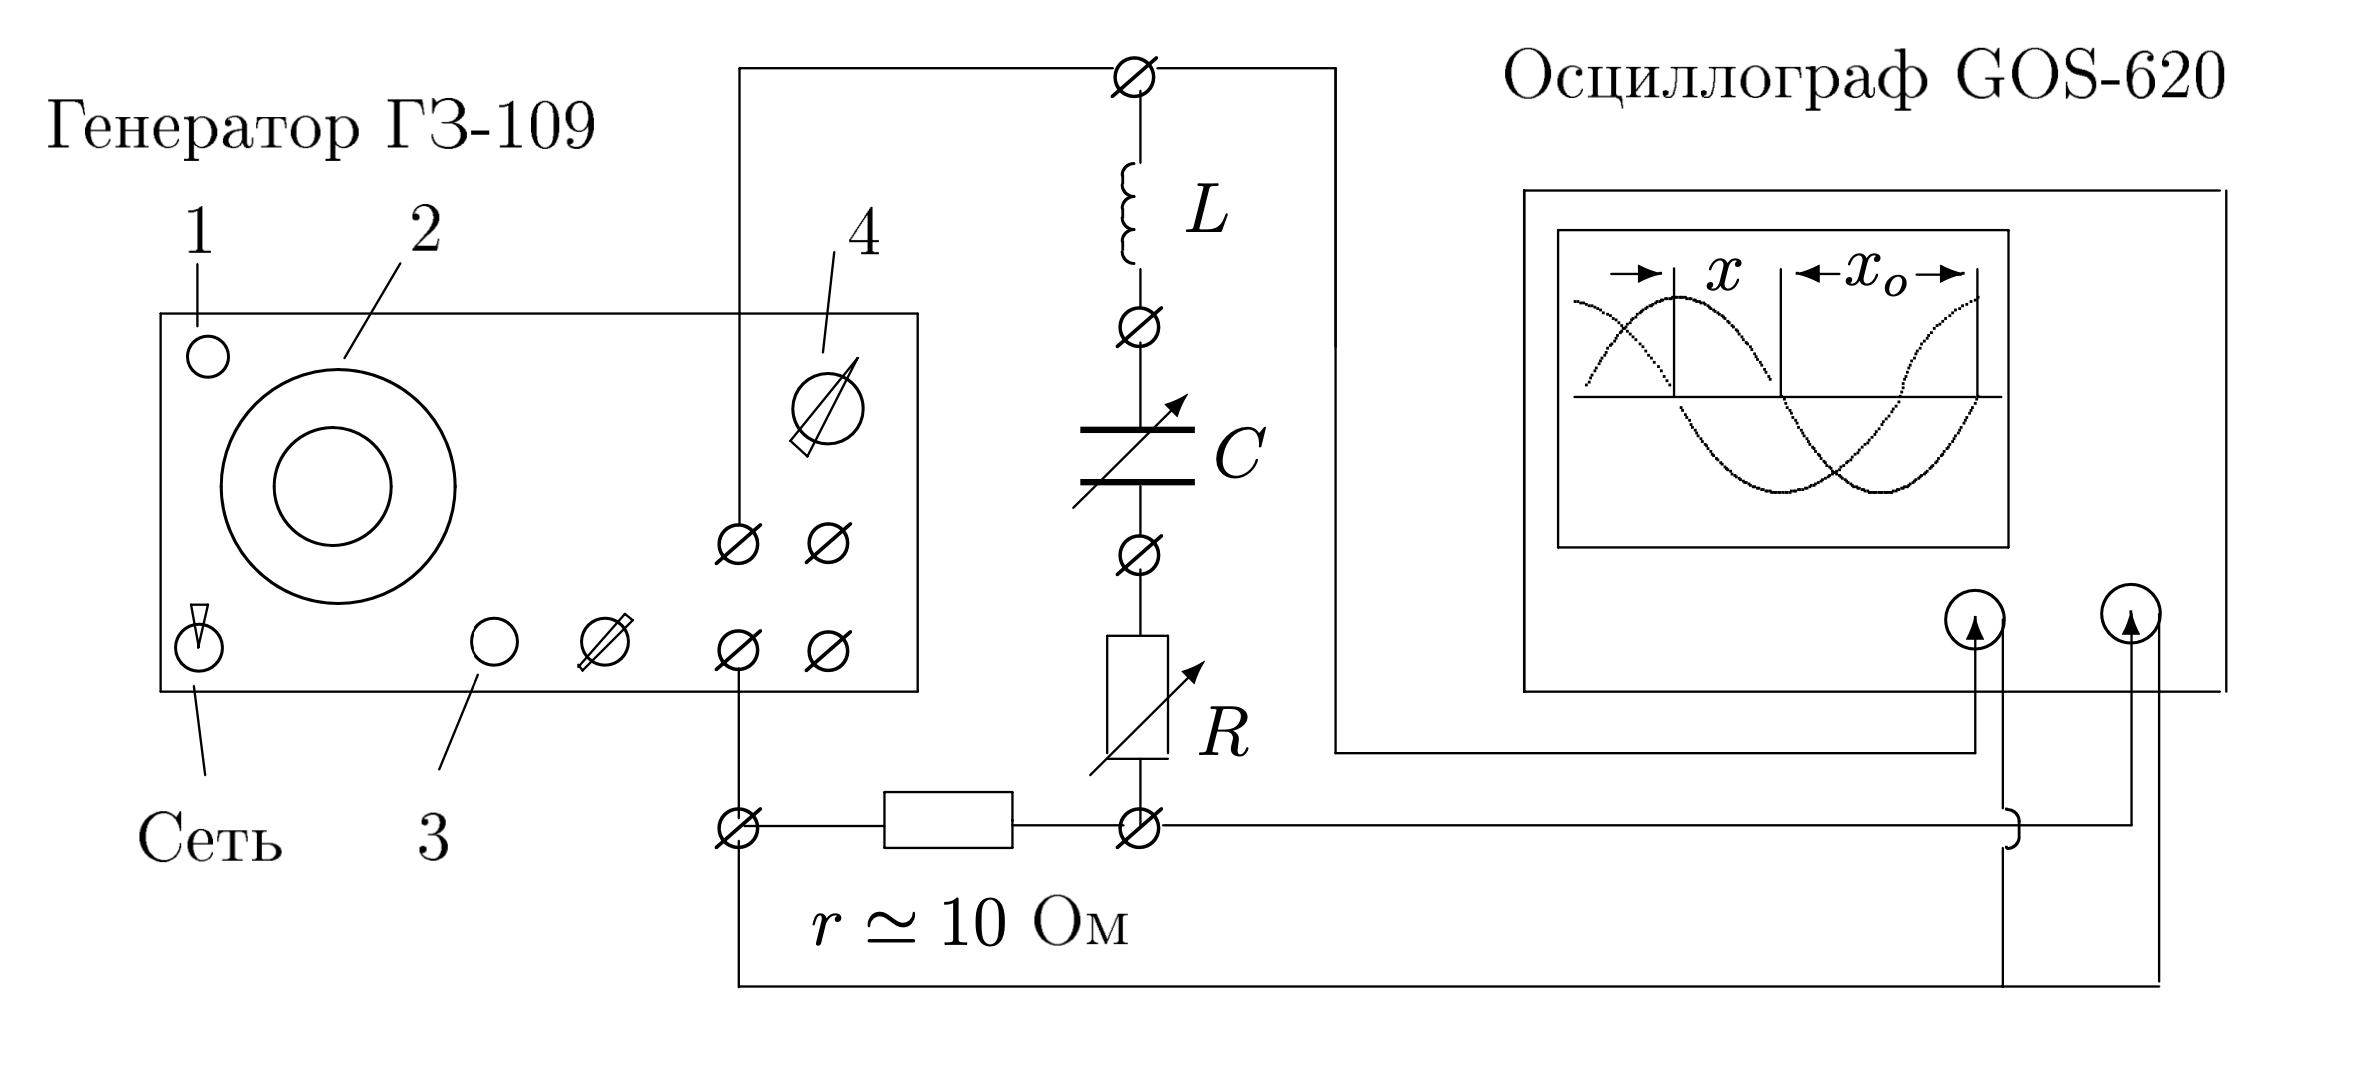
\includegraphics[width=0.7\linewidth]{scheme.png}
    \caption{Схема установки для исседования сдвига фаз между током и напряжением}
\end{figure}

Сигнал, пропорциональный току, снимается c сопротивления $r$, пропорциональный напряжению — с генератора. 
Оба сигнала подаются на универсальный осциллограф. 
Этот осциллограф имеет два канала вертикального отклонения, что позволяет одновременно наблюдать на экране два сигнала. 
В нашей работе это две синусоиды (рис. 3), смещённые друг относительно друга на расстояние x, зависящее от сдвига фаз между током и напряжением в цепи.

Измерение сдвига фаз удобно проводить следующим образом:
     
1) подобрать частоту развертки, при которой на экране осциллографа укладывается чуть больше половины периода синусоиды;
    
2) отцентрировать горизонтальную ось; 

3) измерить расстояние $x_0$ между нулевыми значениями одного из сигналов, что соответствует смещению по фазе на $\pi$;

4) измерить расстояние $x$ между нулевыми значениями двух синусоид и пересчитать в сдвиг по фазе: $\psi = \pi \cdot x/x_0$.

На рис. 1 синусоиды на экране ЭО сдвинуты по фазе на $\pi/2$.

Схема фазовращателя, изображённая на рис. 4, содержит два одинаковых резистора $R_1$, смонтированных на отдельной плате, магазин сопротивлений $R$ и магазин емкостей $C$.

\begin{figure}[h]
    \centering
    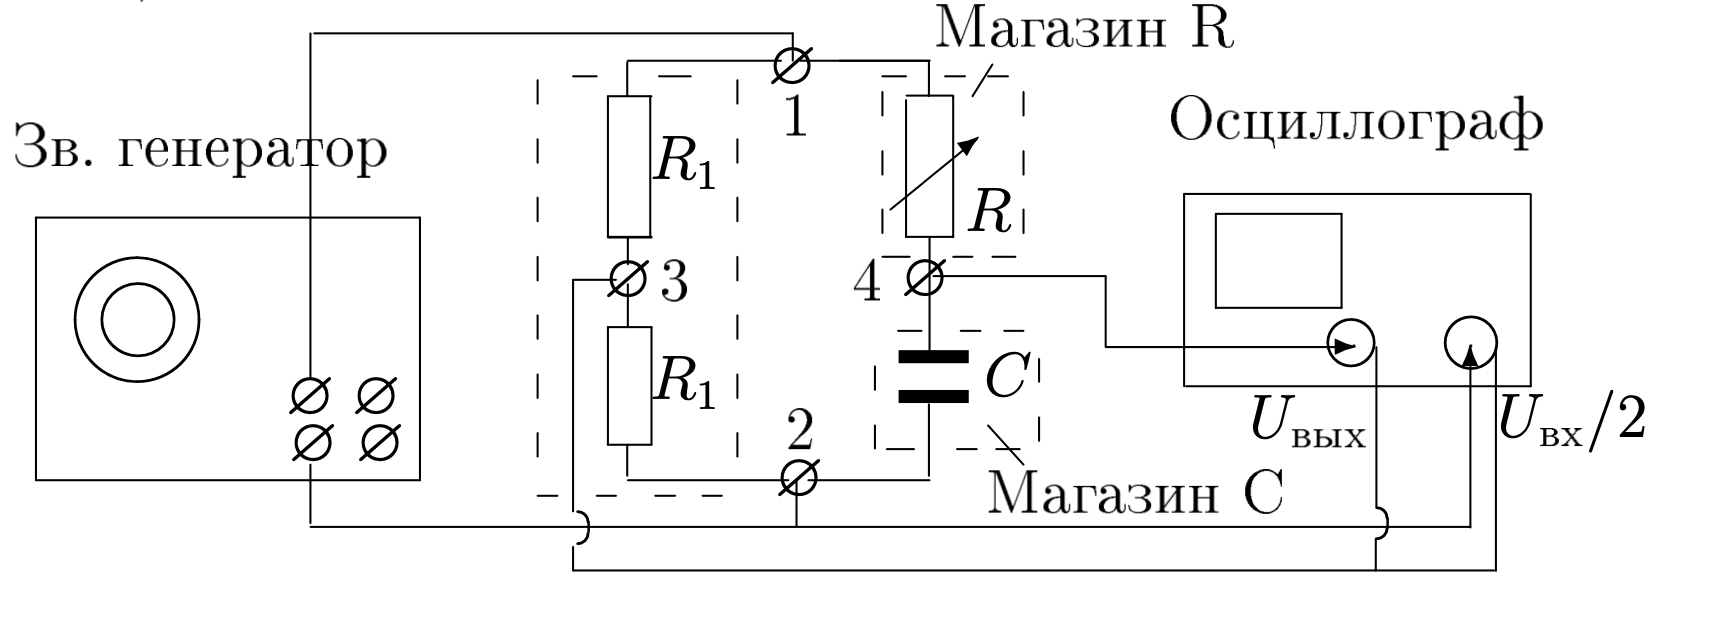
\includegraphics[width=0.7\linewidth]{scheme2.png}
    \caption{Схема установки для исследования фазовращателя}
\end{figure}

\begin{figure}[h]
    \centering
    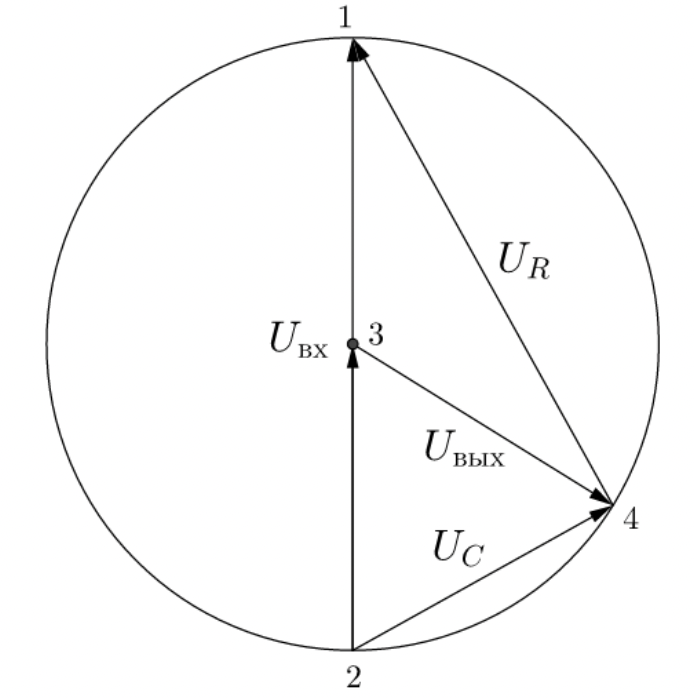
\includegraphics[width=0.4\linewidth]{vectdiagramma.png}
    \caption{Векторная диаграмма фазовращателя}
\end{figure}

Разность фаз равна $\pi/2$, когда медиана 34 является и высотой, т.е. когда $\triangle$124 – равнобедренный.

\subsection*{Результаты измерений и обработка данных}
После сборки схемы (рис. 4) установим на катушке индуктивности максимальное значение $L = 50$ мГн, а в магазине емкостей $C = 0.5$ мкФ, сопротивление $R$ занулим.
На генераторе установим частоту $\nu = 1$ кГц и нагрузку 5 Ом.

Пересоберем схему по рис. 3 и закоротим катушку ($RC-$цепь).

В такой цепи зависимость разности фаз можно вычислить по простой формуле 
\begin{equation}
    \psi = \arctan\left({x \over R_\Sigma}\right),
\end{equation}

где $x = X_L - X_C$ - разность реактивных сопротивлений катушки и конденсантора, \\$R_\Sigma$ - суммарное активное сопротивление цепи.

Реактивное сопротивление в цепи $X_1 = {1\over \omega C} = 31.83$ Ом.
% X1 = 31.831

Будем увеличивать сопротивление $R$ от 0 до $10X_1$ и проведем измерения (табл. 1), подбирая $R$ так, чтобы приращения разности фаз были примерно одинаковы.
\begin{table}[H]
    \centering
    \begin{tabular}{|c|c|c|c|c|c|c|c|}
        \hline
        $R$, Ом &0&40&80&120&190&240&300\\
        \hline
        $\psi$, $2\pi$/50 & 12.5 & 11.5&10.5&9.5&8.5&7.5&6.5\\
        \hline
        % $\psi$, $2\pi$/50 & 37.5 & 38.5&39.5&40.5&41.5&42.5&43.5\\
        % \hline
    \end{tabular}
    \caption{$RC - $цепь}
\end{table}

Изобразим полученные данные на графике (рис. 5) и сравним с теоретическим значением (1).

\begin{figure}[h]
    \centering
    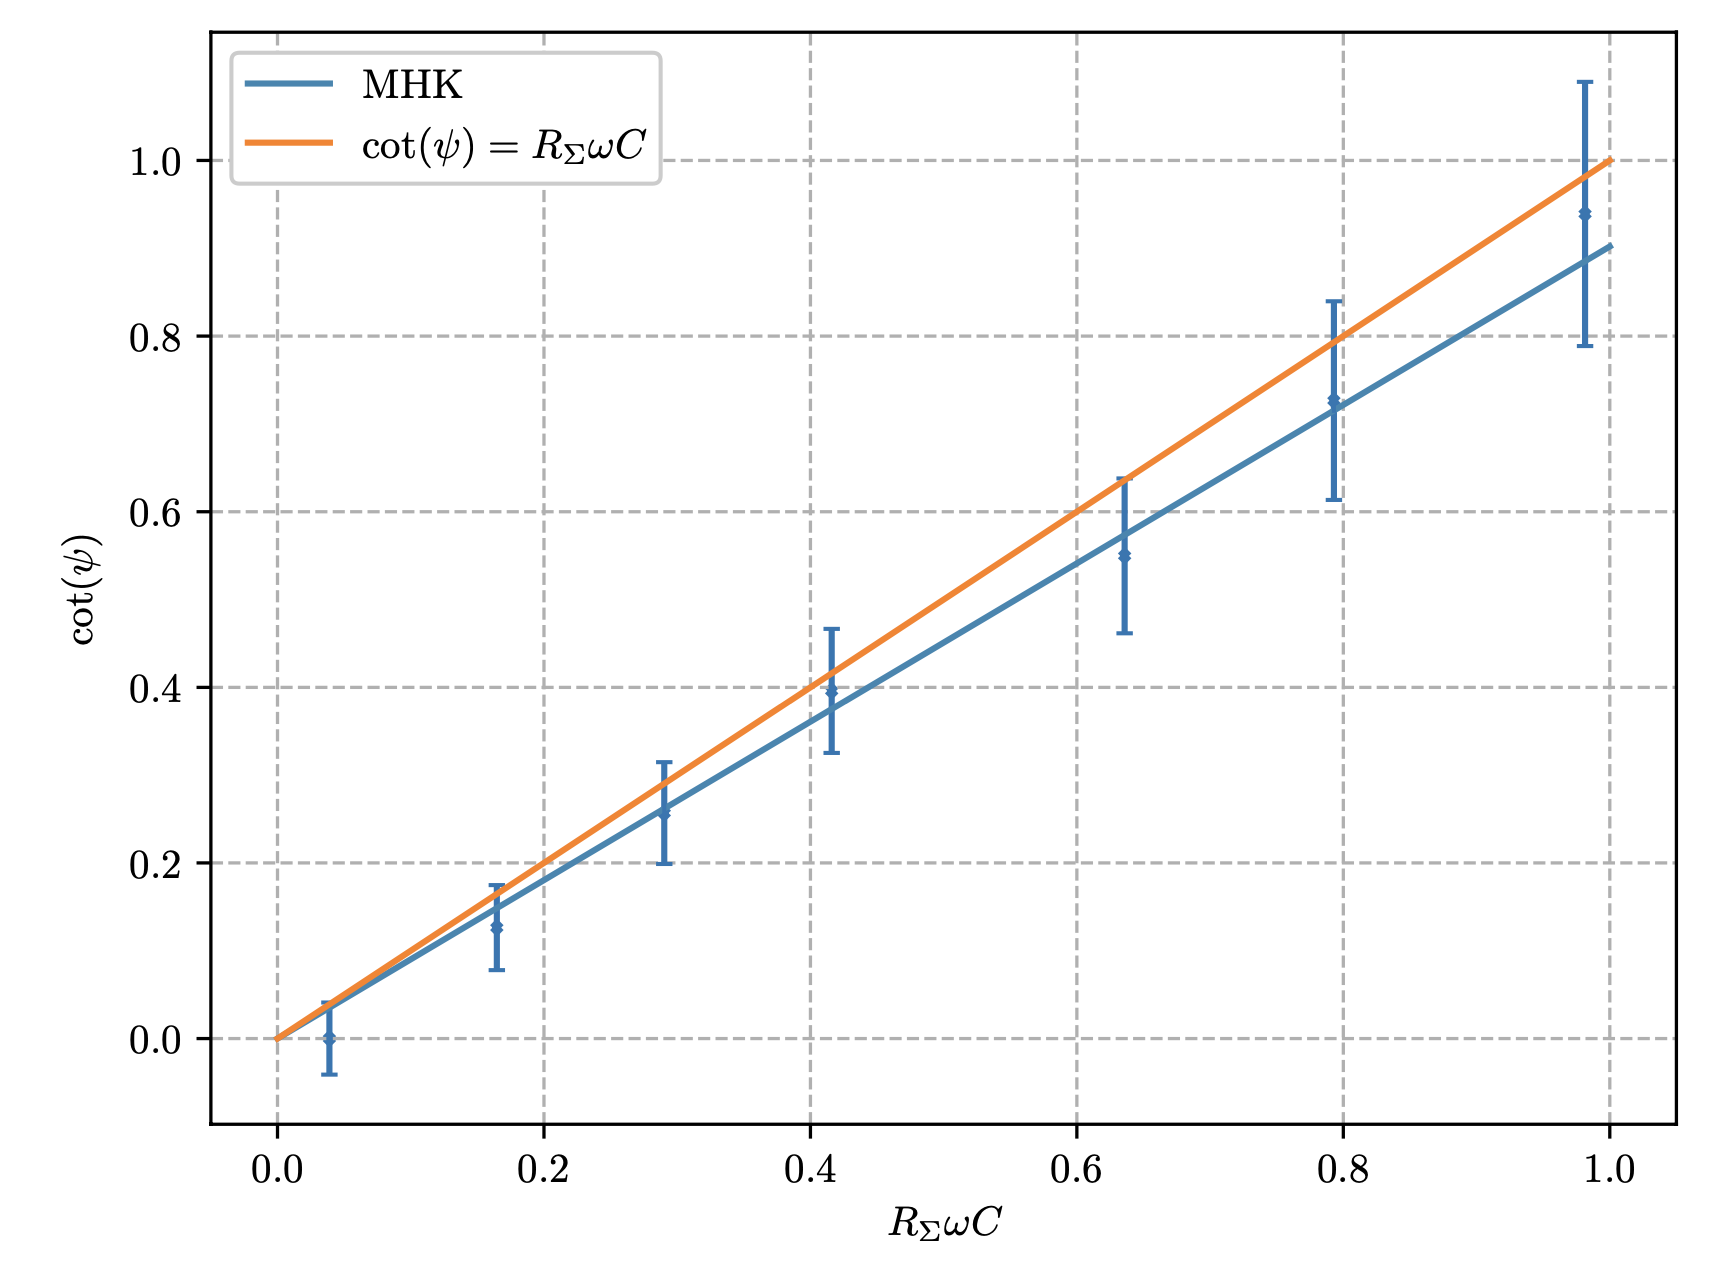
\includegraphics[width=0.6\linewidth]{1.png}
    \caption{Зависимость разности фаз от сопротивления в $RC-$цепи}
\end{figure}

Из графика видно, что измеренные величины довольно хорошо кореллируют с теоретической зависимостью.
По МНК коэффициент наклона $k_c = 0.95 \pm 0.11$, что в пределах погрешности совпадает с теоретическим $k = 1$.
\newpage

Теперь в схеме на рис. 3 закоротим магазин емкостей ($RL-$цепь).

Реактивное сопротивление $X_2 = \omega L = 314.16$ Ом.

Измерим зависимость сдвига фаз от сопротивления (табл. 2), меняя его от 0 до 10$X_2$.


% X2 = 314.16 Ом цепь колеблется!!!!Й
\begin{table}[H]
    \centering
    \begin{tabular}{|c|c|c|c|c|c|c|c|}
        \hline
        $R$, Ом &0&380&700&1100&1500&2000&3000\\
        \hline
        $\psi$, $2\pi$/50 &11.5&5.5&3&2.5&2&1.5&1\\
        % \hline
        % $\psi$, $2\pi$/50 &38.5&44.5&47&47.5&48&48.5&49\\
        \hline
    \end{tabular}
    \caption{$RL - $цепь}
\end{table}

\begin{figure}[H]
    \centering
    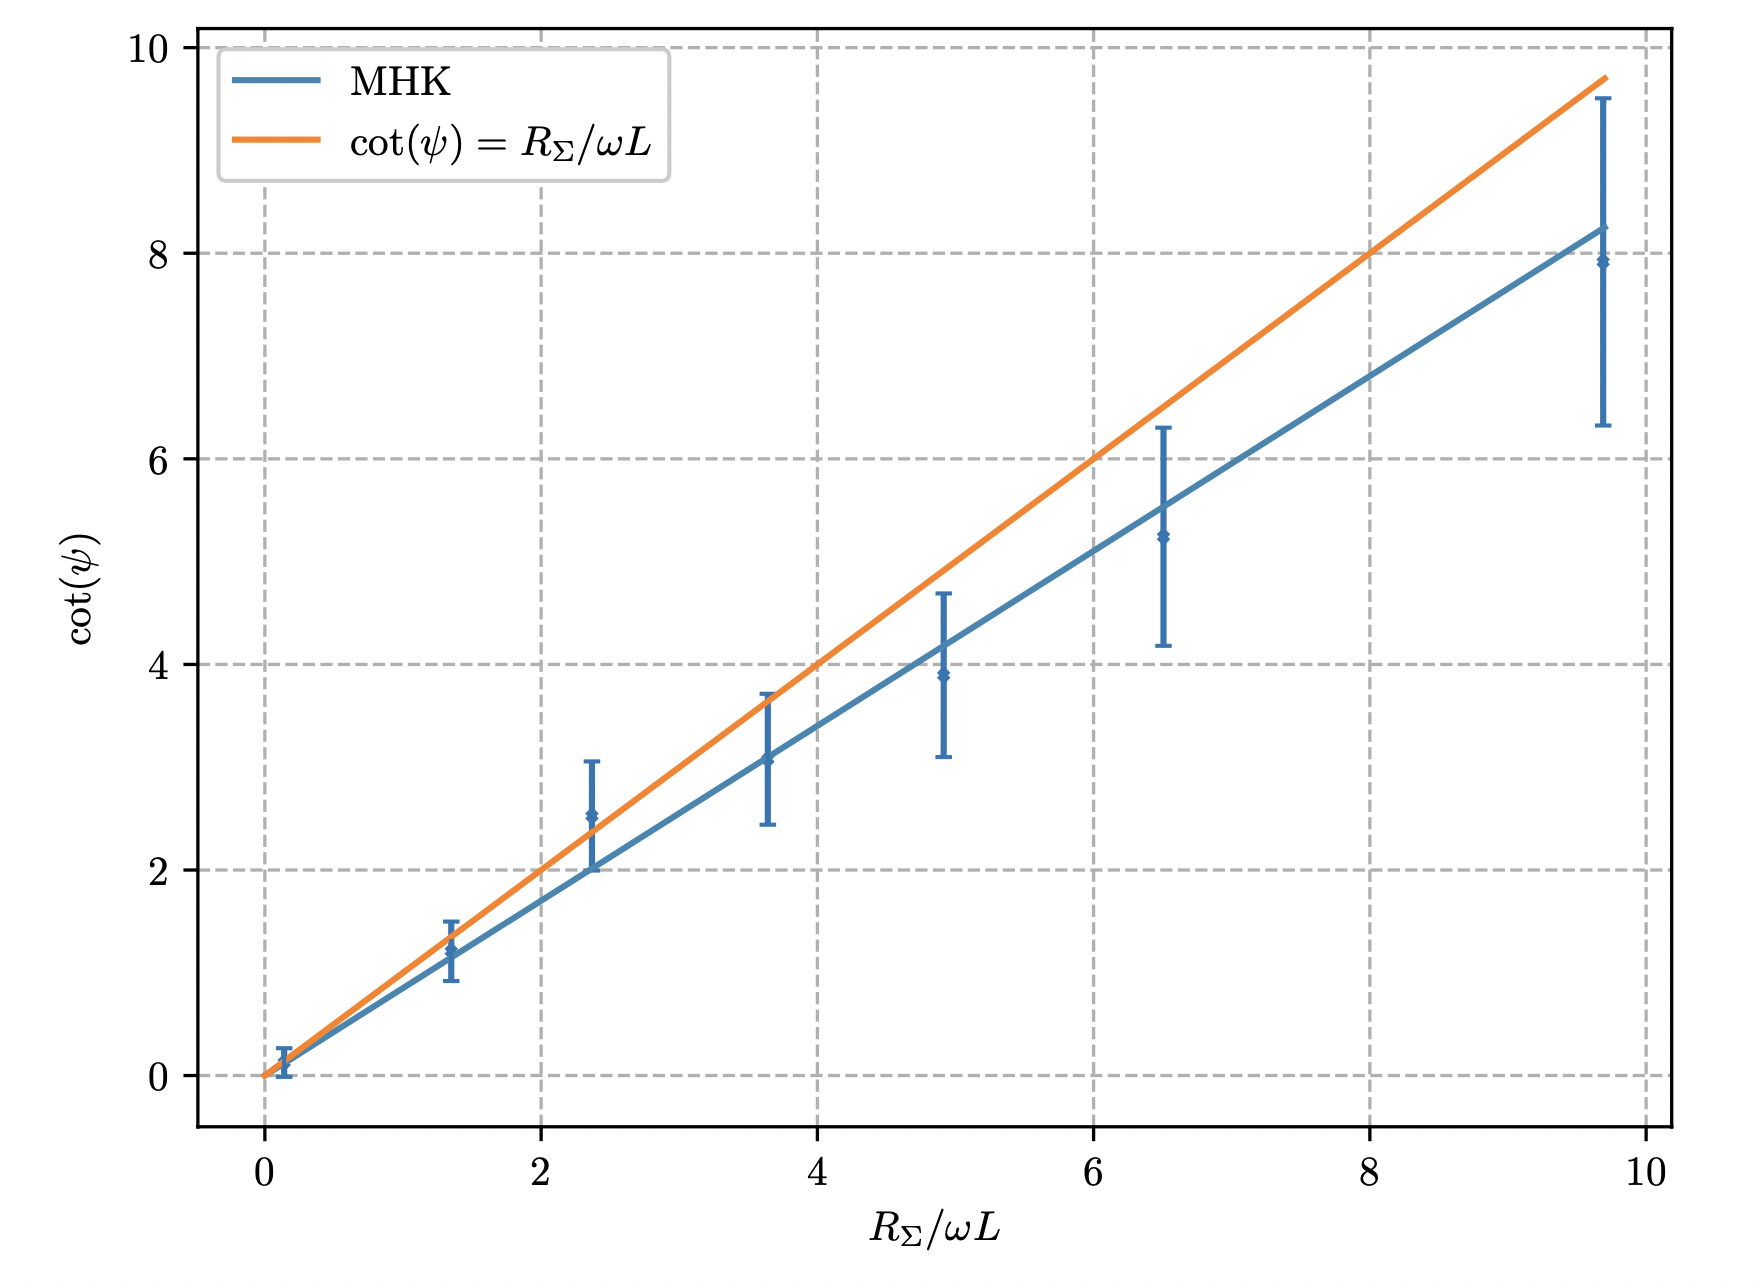
\includegraphics[width=0.6\linewidth]{2.png}
    \caption{Зависимость разности фаз от сопротивления в $RL-$цепи}
\end{figure}

По МНК $k = 0.89 \pm 0.13$, что в пределах погрешности совпадает с теоретическим $k = 1$.
\newline

Теперь проведем измерения в $RLC-$цепи.

Резонансная частота $\nu_0 = {2\over 2\pi \sqrt{LC}} = 1006.58$ Гц.
Теоретически полученное значение: $\nu_0 \approx 990$ Гц.

Снимем зависимость сдвига фаз (от $-\pi/3$ до  $\pi/3$) от частоты (табл. 3) при $R = 0$ и при $R=100$ Ом.
% R(-1/3) = 890, R(1/3) = 1120 (верхняя строка R = 0, нижняя R = 100 Ом)
\begin{table}[H]
    \centering
    \begin{tabular}{|c|c|c|c|c|c|c|c|}
        \hline
        \multicolumn{8}{|c|}{$R = 0$} \\
        \hline
        $\nu$, Ом &890&930&970&990&1040&1080&1120\\
        \hline
        $x/x_0$ &-1/3&-9/35&-4/33&0&1/5&8/29&1/3\\
        \hline
        \multicolumn{8}{|c|}{$R = 100$ Ом} \\
        \hline
        $\nu$, Ом &700&800&900&990&1100&1200&1400\\
        \hline
        $x/x_0$ &-7/22&-5/19&-5/34&0&1/12&3/13&7/22\\
        \hline
    \end{tabular}
    \caption{$RCL - $цепь}
\end{table}

Изобразим данные на одном графике (рис. 7)

\begin{figure}[H]
    \centering
    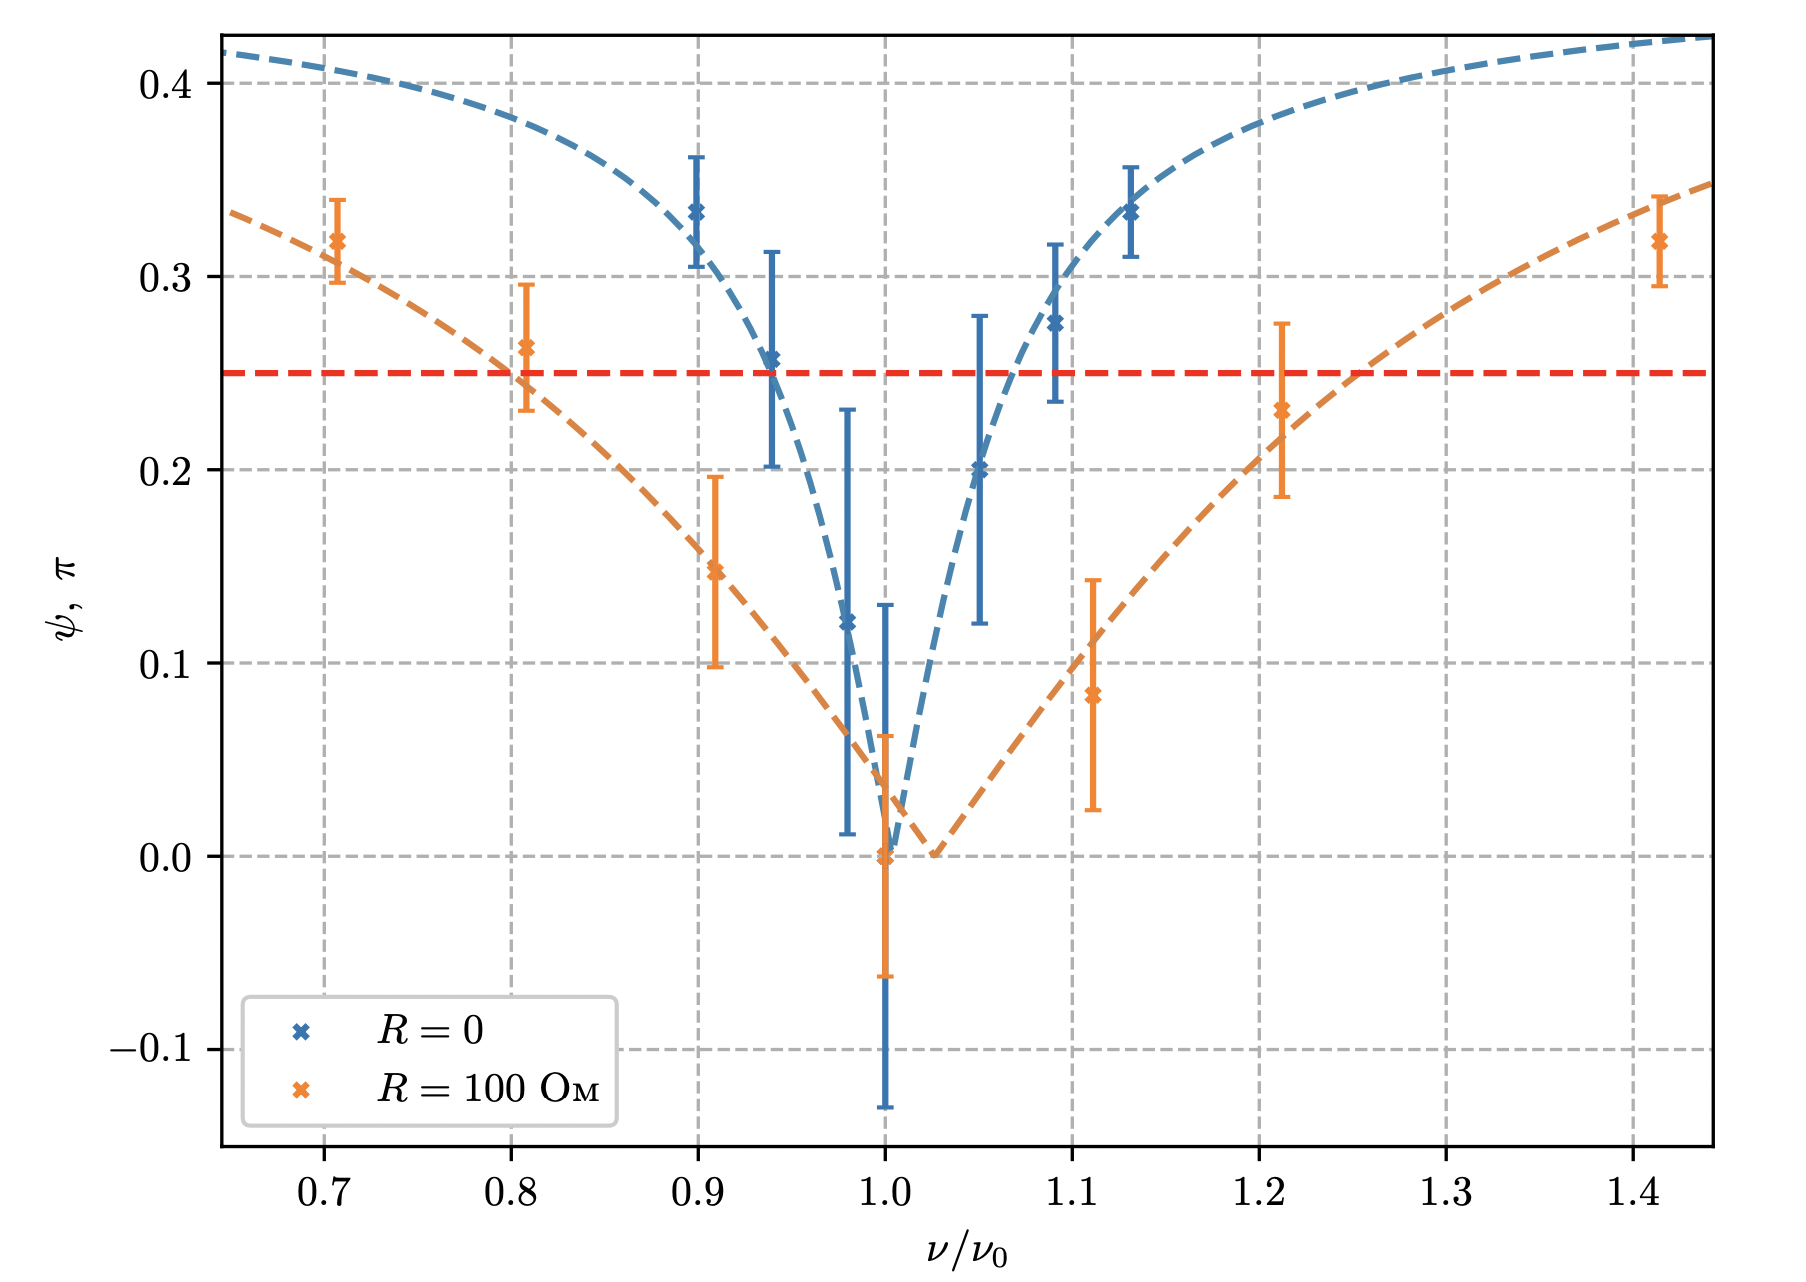
\includegraphics[width=0.7\linewidth]{3.png}
    \caption{Зависимость разности фаз от частоты}
\end{figure}

При сдвиге фаз $\psi = \pi/4$ ширины графиков равны соответственно %0.135 и 0.430. 
0.128 и 0.434
Тогда добротности схем равны $Q_{прак}(0) = 7.8,\ Q_{прак}(100) = 2.3$.

Также запишем параметры установки:
сопротивление $r = 12.4$ Ом, индуктивность $L = 50$ мГн и активное сопротивление $R_L = 31.5$ Ом.


Теоретически добротность контура равна 
\begin{equation*}
    Q = {1 \over R_\Sigma} \sqrt{L \over C}.
\end{equation*}

Тогда при $R = 0$ $Q_{теор} = 7.2$, при $R = 100$ Ом $Q_{теор} = 2.2$, что примерно совпадает с экспериментальными значениями.
\newline

Соберем установку по рис. 4 и оценим диапазон изменения сдвига фаз при $\nu = 1$ кГц и $C = 0.5$ мкФ: он меняется от $\psi(0) = 0$ до $\psi(10кОм) = \pi/2$.

\subsection*{Подведение итогов}
В ходе работы исследована зависимость сдвига фаз между током и напряжением от сопротивления. 
В $RC-$ и $RL-$ цепях экспериментальные значения в пределах погрешности совпадают с теоретическими.


Также определена добротность колебательного контура путем снятия зависимости сдвига фаз от частоты вблизи резонанса: для $R = 0$ значение $Q = 7.8$, что примерно совпадает с теоретическим $Q=7.2$ ($\varepsilon \approx 9\%$), для $R=100$ Ом добротность контура $Q = 2.3$, что также хорошо кореллирует с теоретическим значением $Q = 2.2$ ($\varepsilon \approx 5\%$).
\end{document}